\section{Revised Solution Design}
\label{sec:revised_solution_design}

The Basilisk platform is missing some key functionality to successfully run benchmark jobs.
In this section we describe the designed solutions for the shortcomings listed in section \ref{sec:architecture_review}.



\subsection{Code Refactoring}
\label{sec:impl_code_refactor}
As stated in section \ref{sec:code_refactor}, an in-depth code refactoring was recommended.
Before starting to design and implement new functionality, we performed an in-depth refactoring and restructuring of the code base.
This created a clean code base on which all future implementations can be build on.

Code refactoring is the process of restructuring the source code of an application without changing its functionality\cite{fowlerRefactoringImprovingDesign2019a}.


\subsection{Management of Repositories and Configurations}
\label{sec:management_repo_config_design}
Section \ref{sec:management_repo_config} already explains the problem of storing and managing repositories, the corresponding hooks and the \ts{}-configurations between the \acf{hcs} and the \acf{jms}.

We discussed different possible solutions, of moving functionality or merging the functionality of the two services into one.
\todo[inline,color=green]{Ist so ein Satz okay der den Denkprozess erklärt? oder nur das Ergebnis erklären?}

In the designed solution, the management and storing of the repositories is moved into the \ac{jms}.
This includes the corresponding REST endpoints and internal logic of the \ac{hcs} that are needed for the management.
The different repositories (\gh{} and \dockh{}) will then be added over the REST API of the \ac{jms}.

In section \ref{sec:review_missing_impl} (\acl{hcs}) it is listed, that the \ac{hcs} is missing the REST endpoints for deleting repositories.
Since the repository management is moved to the \ac{jms}, these endpoints also need to be added there.
\\

The \ac{jms} will communicate with the \ac{hcs} over RabbitMQ message queues.
Through these messages the \ac{hcs} will get the needed information about the repositories it should observe.
These include the URL and for \gh{} repositories details like the observed branch and potentially an OAuth token.

The functionality used when a new release is found, does not need to be changed.
When a new release is found, the \ac{hcs} still sends a message containing the relevant information to the \ac{jms}.
\\

Figure \ref{fig:repo_management_restructure} shows the restructured REST APIs and the adjusted messaging between \ac{hcs} and \ac{jms}.

\begin{figure}[tbph]
	\centering
	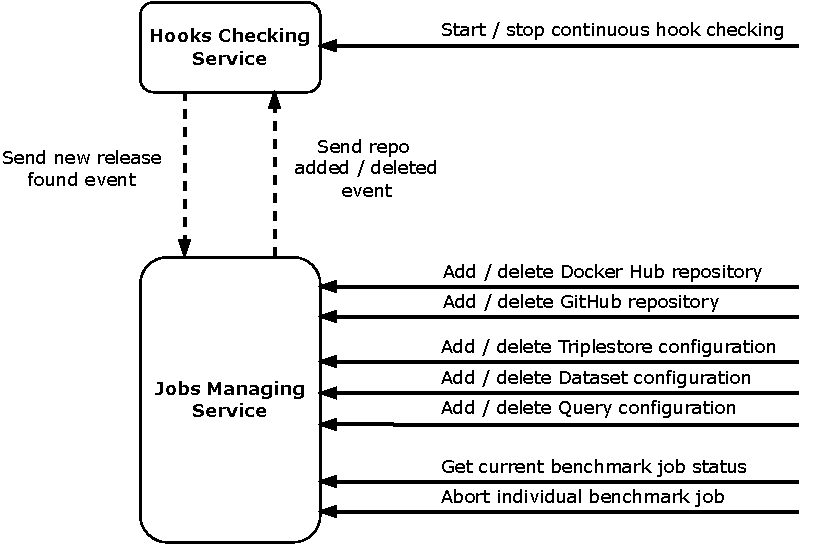
\includegraphics[width=.65\textwidth]{figures/messaging-implementation-hcs-jms.pdf}
	\caption{Overview of the restructured REST APIs and adjusted messaging}
	\label{fig:repo_management_restructure}
\end{figure}



\subsection{Restructure of Data Models in the \acl{jms}}
\label{sec:data_model_restructure_jms}
In section \ref{sec:review_data_model} we reviewed the data model used for storing and managing the different configuration types inside the \ac{jms}.
To mitigate the stated problems with the data model, we designed the database schema shown in figure \ref{fig:design_jms_db_schema}.

\begin{figure}[tbph]
	\centering
	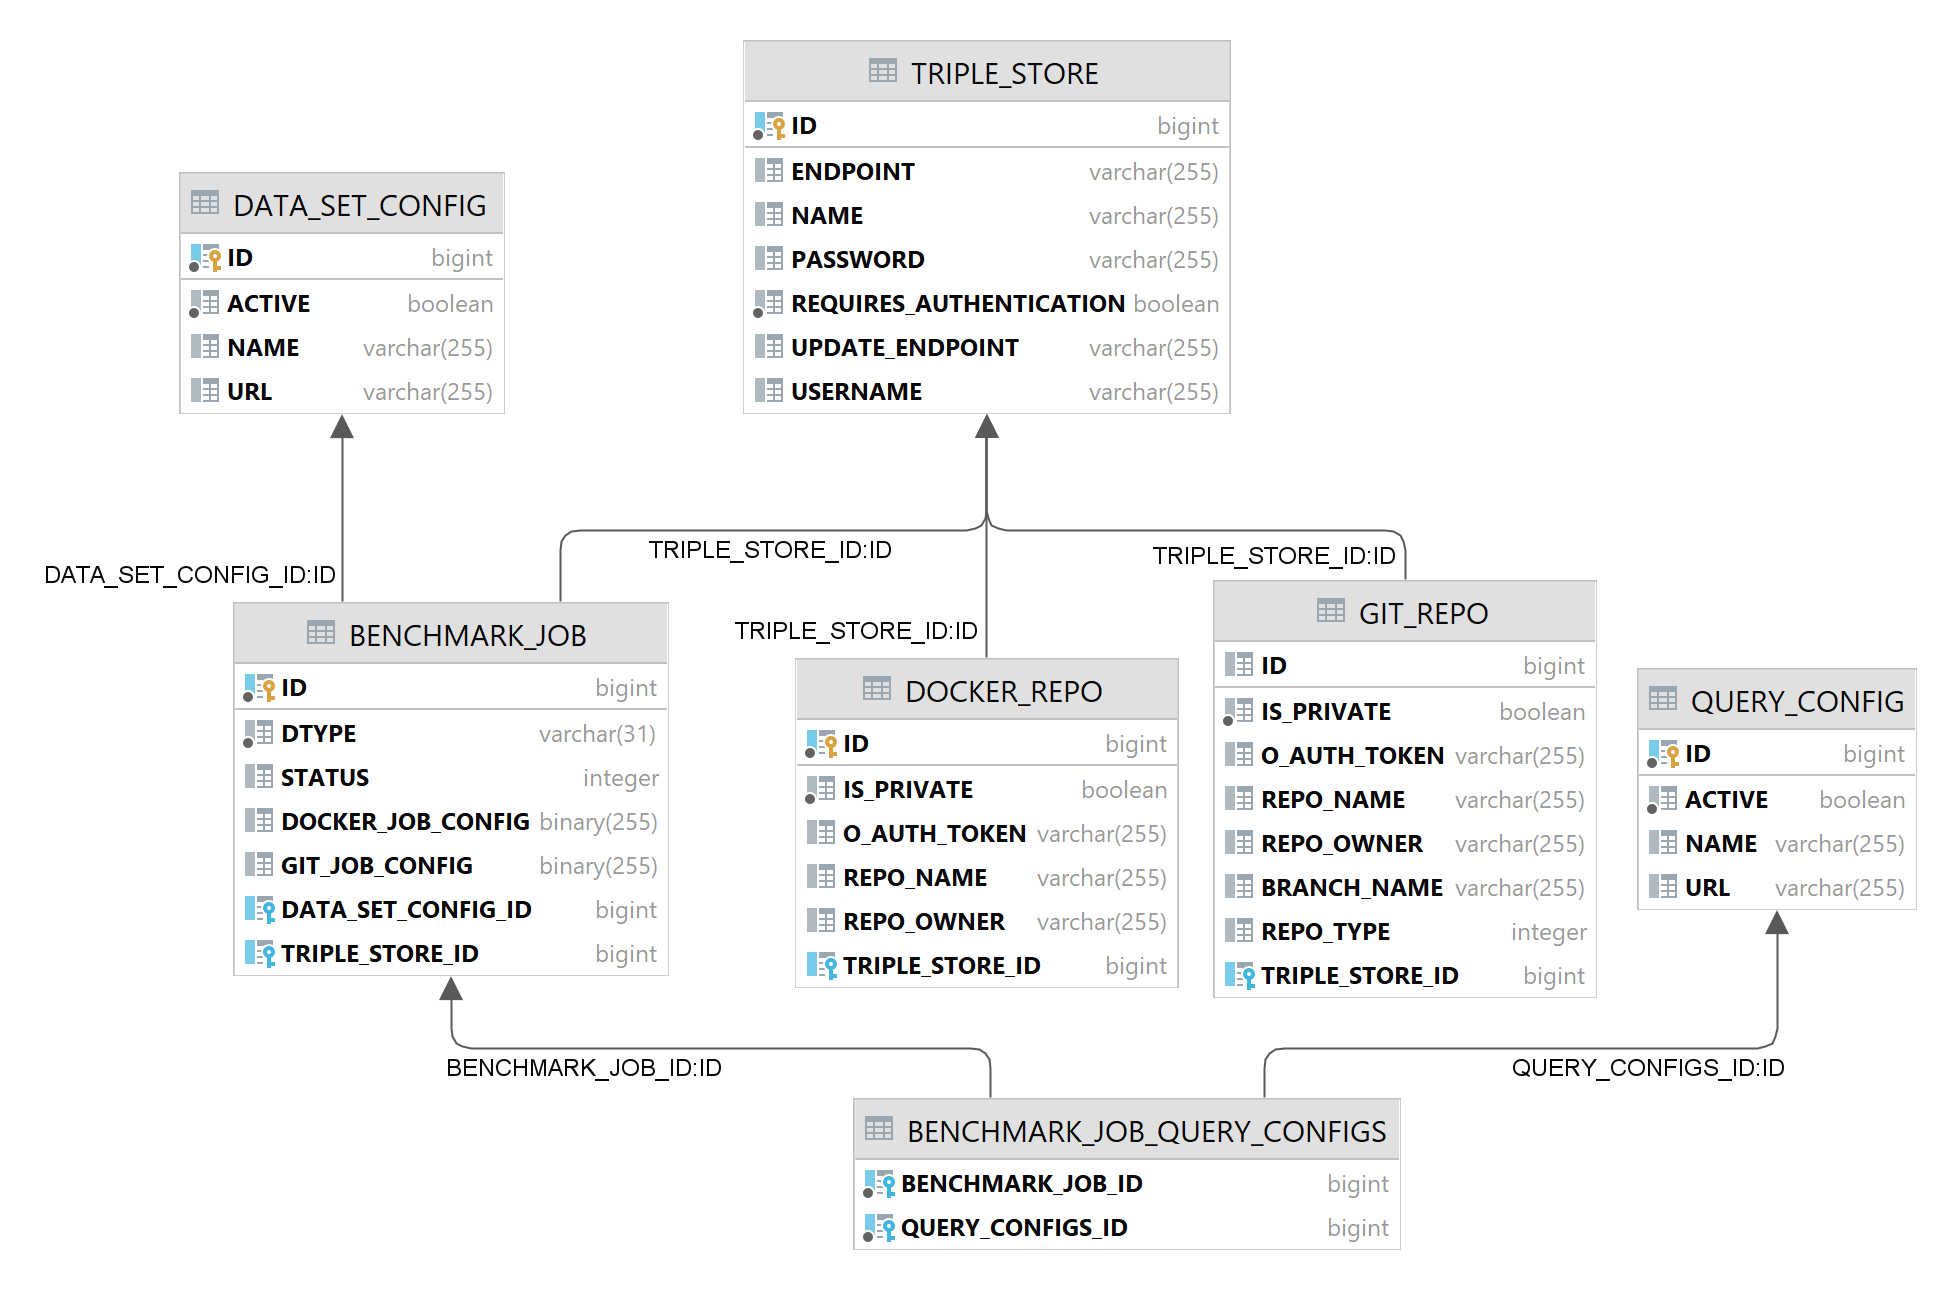
\includegraphics[width=.95\textwidth]{figures/jms_db_schema_design.png}
	\caption{Diagram of the proposed database schema for the \ac{jms}}
	\label{fig:design_jms_db_schema}
\end{figure}

In this design we introduce two different repository types.
One for \gh{} and one for \dockh{}.
This ensures that a repository is always correctly referenced when creating a new benchmark job.

Secondly the relationship between \ac{ts} configurations and repositories is inverted. 
Now each setup repository points to a \ac{ts} configuration.
This means a \ac{ts} configuration can be used for different observed repository setups.

\todo[inline]{changes to benchmark job and dataset/query configs?}


\subsection{Hooks for Pull Requests in \gh{} Repositories}
Currently the Basilisk platform can not check for new pull request published to an observed repository.
This functionality would greatly support the continuous benchmarking during the development process of \tsp{}.

As explained in chapter \ref{ch:approach}, \tsp{} are often developed by teams who collaboratively work on Git repositories.
A standard way of introducing a newly developed feature to a source code repository is a pull request.
Pull requests contain a description of the proposed changes, as well as the name of the development branch which should be pulled into the main branch of the repository.

Often these changes are developed in a forked repository.
A forked repository is basically an independent copy of the main repository.
\gh{} provides functionality to merge the latest changes of the original repo into the forked repo.
To send changes from the forked repo to the original repo, a pull request is needed.

In this forked repo the developer can work independently on his changes and later create the pull request to the original repository.

The difficulty for the Basilisk platform is, that these pull requests can stem from these forked repositories.
Since the repository containing the changes has a different URL to the original repo observed by the Basilisk platform, more information than usual are required to create and run a benchmark job for a pull request.
\\

The solution we designed for this issue is an extended message.
This message gets send in the situation in which the pull requests originates from a different repository.
The message contains the URL, repository and branch name for the \gh{} repository.
Therefore the message handling in the \ac{hcs} and \ac{jms} needs to be adjusted to handle this new message type.

The benchmark jobs and the \acl{tbs} does not need to be changed.
It is not relevant for a benchmark if the repository, from which the docker container is build, is different too the observed repository.


\subsection{Missing Implementations}
\todo[inline,color=green]{Soll ich auch beschreiben, wie ich die fehlenden REST APIs "designed" habe? Oder reicht kurzer Text im Implementation Teil?}
- JMS extend APIs?

- TBS design docker setup flow??


